\documentclass{article}
\usepackage{setspace,tikz,wrapfig}
\usepackage[text={6.5in,8.5in},centering]{geometry}
\geometry{verbose,a4paper,tmargin=2.4cm,bmargin=2.4cm,lmargin=2.4cm,rmargin=2.4cm}
\usepackage{graphicx,amsmath,cases,multirow,appendix,graphicx,xcolor}
\usepackage[makeroom]{cancel}

\setlength\parindent{0pt}

\newcommand{\note}[1]{\colorbox{gray!30}{#1}}
\newcommand{\ind}{\-\hspace{1cm}}
\newcommand*\circled[1]{\tikz[baseline=(char.base)]{
            \node[shape=circle,draw,inner sep=2pt] (char) {#1};}}
\newenvironment{rcases}
  {\left.\begin{aligned}}
  {\end{aligned}\right\rbrace} 
  
  
\renewcommand\floatpagefraction{.9}
\renewcommand\topfraction{.9}
\renewcommand\bottomfraction{.9}           


\begin{document}

\noindent\makebox[\textwidth][c]{\Large\bfseries Lecture 15 -- Network modules (3-spp.)}

\textbf{Today's models:}\\
\ind - Competition for explicit resources\\
\ind - Trophic chain\\
\ind - Intraguild predation

\textbf{Concepts:}\\
\ind - Competitive exclusion principle (niche partitioning)\\
\ind - Determining invasibility and coexistence criteria\\
\ind - Temporal niche partitioning (Armstrong-McGehee effects)

\rule[0.5ex]{\linewidth}{1pt}
\begin{center}
	\textbf{Exploitative Competition for Explicit Resource}
\end{center}

\textbf{Recall}: 2-spp. LV competition with implicit resource\\
\ind $\Rightarrow$ Intra $>$ Inter-specific competition for coexistence\\
\ind Same general insight from $n$-spp. community matrix analysis.\\

\textbf{Today}: Start with 2 species competing for explicit resource.\\
\ind Include self-limitation in resource\\
\ind  (Know that strong self-limitation on some species is needed for stable coexistence to be possible).
\begin{align*}
	\frac{dO}{dt}&=\overbrace{e_{RO}a_{RO}R O}^{\text{linear intxn}} - \overbrace{m_o O}^{\text{exponential}}\\
	\frac{dC}{dt}&=e_{RC}a_{RC}RC - m_c C\\
	\frac{dR}{dt}&=r R \left(1-\frac{R}{K}\right) - a_{RC}RC - a_{RO}RO
\end{align*}

Today's class is going to be \emph{`Active learning'} style\\
\ind \note{Groups of ~4-5 people.  (1 whiteboard per group.)}\\

Use the methods we've learned in class to answer (\note{referring to notes is okay})...\\
\note{Questions:}
\begin{enumerate}
	\item How many equilibria exist?
	\item What are they (symbolically)?
	\item Which are stable/unstable?
\end{enumerate}
In other words: \textbf{How can both species coexists on a single resource?}\\
\ind \note{Hint:  Best to start analysing $\frac{dO}{dt}$ and $\frac{dC}{dt}$ rather than $\frac{dR}{dt}$}.\\
\ind $\Rightarrow$ Graphical analysis of isoclines.\\

\note{Let groups work for ~20 min.(?) before volunteer group explains to rest, or work through it together.}

\rule[0.5ex]{\linewidth}{1pt}
\pagebreak

\note{Answer:}\\
In order for a species to invade, its per capita growth rate must be positive:  $\frac{1}{N}\frac{dN}{dt}>0$\\

Predator isoclines: (Note really \emph{isoclines}, but rather \emph{`isoplanes'}.)
\begin{align*}
	\frac{1}{O}\frac{dO}{dt} = e_{RO}a_{RO}-m_0 = 0 & \qquad \Rightarrow  \qquad R_O^* = \frac{m_O}{e_{RO}a_{RO}}\\
	\frac{1}{C}\frac{dC}{dt} = e_{RC}a_{RC}-m_C = 0 & \qquad \Rightarrow  \qquad R_C^* = \frac{m_C}{e_{RC}a_{RC}}
\end{align*}
Prey isocline(s):
\begin{align*}
	\frac{dR}{dt}=rR\left(1-\frac{R}{K}\right) = a_{RC}RC + a_{RO}RO = 0  & \qquad \Rightarrow  \qquad r-\frac{rR}{K}-a_{RC}C - a_{RO}O\\
	& \qquad \Rightarrow  \qquad O_R^* = \frac{r-\tfrac{rR}{K}-a_{RC}C}{a_{RO}}\\
	& \qquad \Rightarrow  \qquad C_R^* = \frac{r-\tfrac{rR}{K}-a_{RO}O}{a_{RC}}\\
\end{align*}
Note that $O_R^*$ and $C_R^*$ are linearly declining functions of both $R$ and $C/O$.

Look at marginal view of phase portrait (i.e. 3D in 2D):
\begin{center}
 	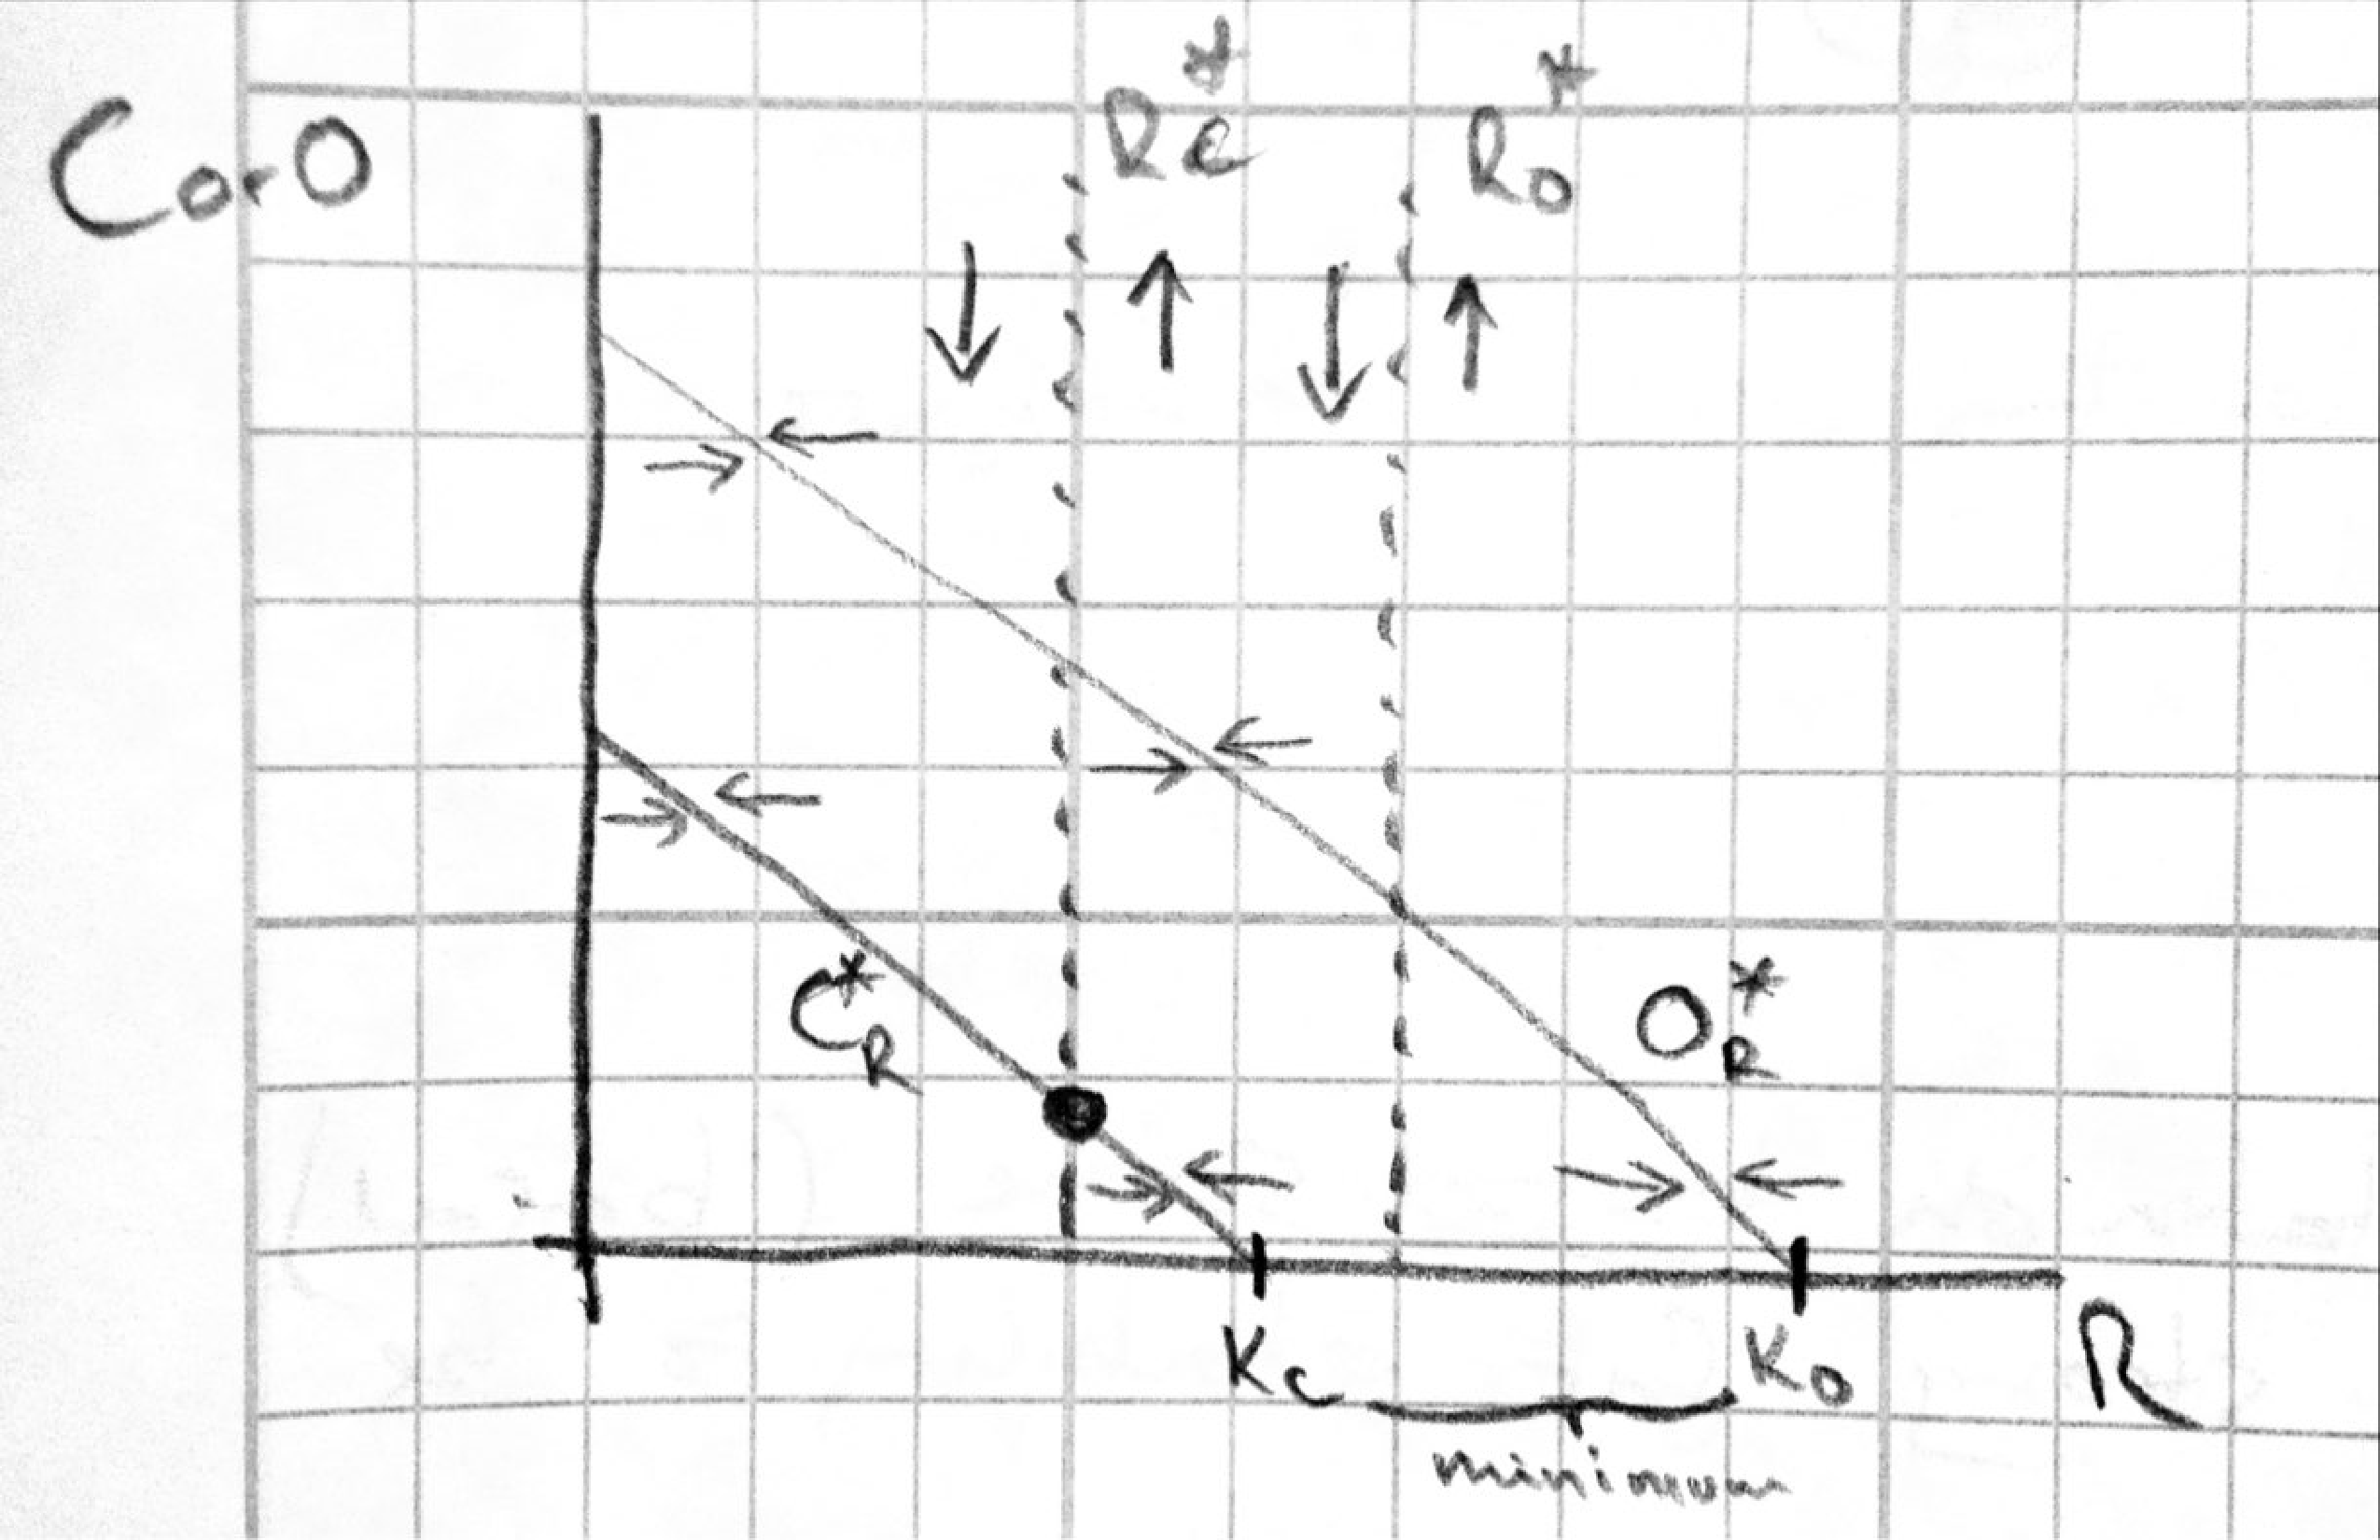
\includegraphics[width=10cm]{figs/LVcomp.pdf}
\end{center}

\textbf{Conclusions:}
\begin{enumerate}
\item $K_C$ and $K_O$ are minimum carrying capacities needed for coexistence of either consumer with $R$.
\item* Whichever species has the lower $R^*$ out-competes the other!
\item $R^*$ is a metric for competitive superiority.\\
\ind $C$ out-competes $O$ if $R_C^* < R_O^*$ ...which means that $m_C < m_O$ and/or $e_{RC} a_{RC} > e_{RO} a_{RO}$.

\item Competitive exclusion occurs regardless of carrying capacity ($K$ doesn't show up in either $R_i^*$).\\
\ind As long as $K>\min R_i^*$, there will be only 1 consumer species.\\
\end{enumerate}
\textbf{But note assumption of linear species intxns.}  (Will get back to this.)

\rule[0.5ex]{\linewidth}{1pt}
\pagebreak
\begin{center}	\textbf{Trophic Chain} \end{center}
\begin{align*}
		\frac{dO}{dt}&=e_{CO}a_{CO}C O - m_o O\\
		\frac{dC}{dt}&=e_{RC}a_{RC}R C -a_{CO}CO- m_c C\\
		\frac{dR}{dt}&=r R \left(1-\frac{R}{K}\right) - a_{RC}RC
\end{align*}

Intuition from previous (exploitative competition) model:\\
\ind Need some minimum amount of energy/productivity to support higher trophic levels.\\
\ind Since middle-school probably know that ~90\% of energy is lost at each trophic transfer.\\

\note{Questions:}
\begin{enumerate}
	\item How many equilibria and what are they (\emph{qualitatively})?
	\item What level of productivity ($K_i$) allows each consumer to invade (\emph{symbolically})?
\end{enumerate}

\circled{1} Trivial equilibrium $\Rightarrow R_{eq}^*=C_{eq}^*=O_{eq}^*=0$\\

\circled{2} Resource-only $\Rightarrow R_{eq}^* = K$\\

\circled{3} When can $C$ invade $R$-only system?\\
\ind In order to invade $\frac{1}{C}\frac{dC}{dt}>0$.\\
\ind Consumer isocline:
\begin{align*}
	\frac{1}{C}\frac{dC}{dt}=e_{RC}a_{RC} R -\cancelto{0}{a_{CO}CO} - m_C  = 0 \qquad \Rightarrow \qquad R_C^* =\frac{m_C}{e_{RC}a_{RC}}
\end{align*}
\ind Resource isocline:
\begin{align*}
	\frac{dR}{dt}=rR-\frac{rR^2}{K}-a_{RC}RC = 0 \qquad \Rightarrow \qquad C_R^* = \frac{r-\frac{rR}{K}}{a_{RC}}
\end{align*}
\ind Conclusion:\\
\ind \ind $C$ can invade when $K\geq R_C^*$.\\
\ind \ind The $R$-only system becomes \emph{unstable} when $K\geq R_C^*$.
\begin{center}
 	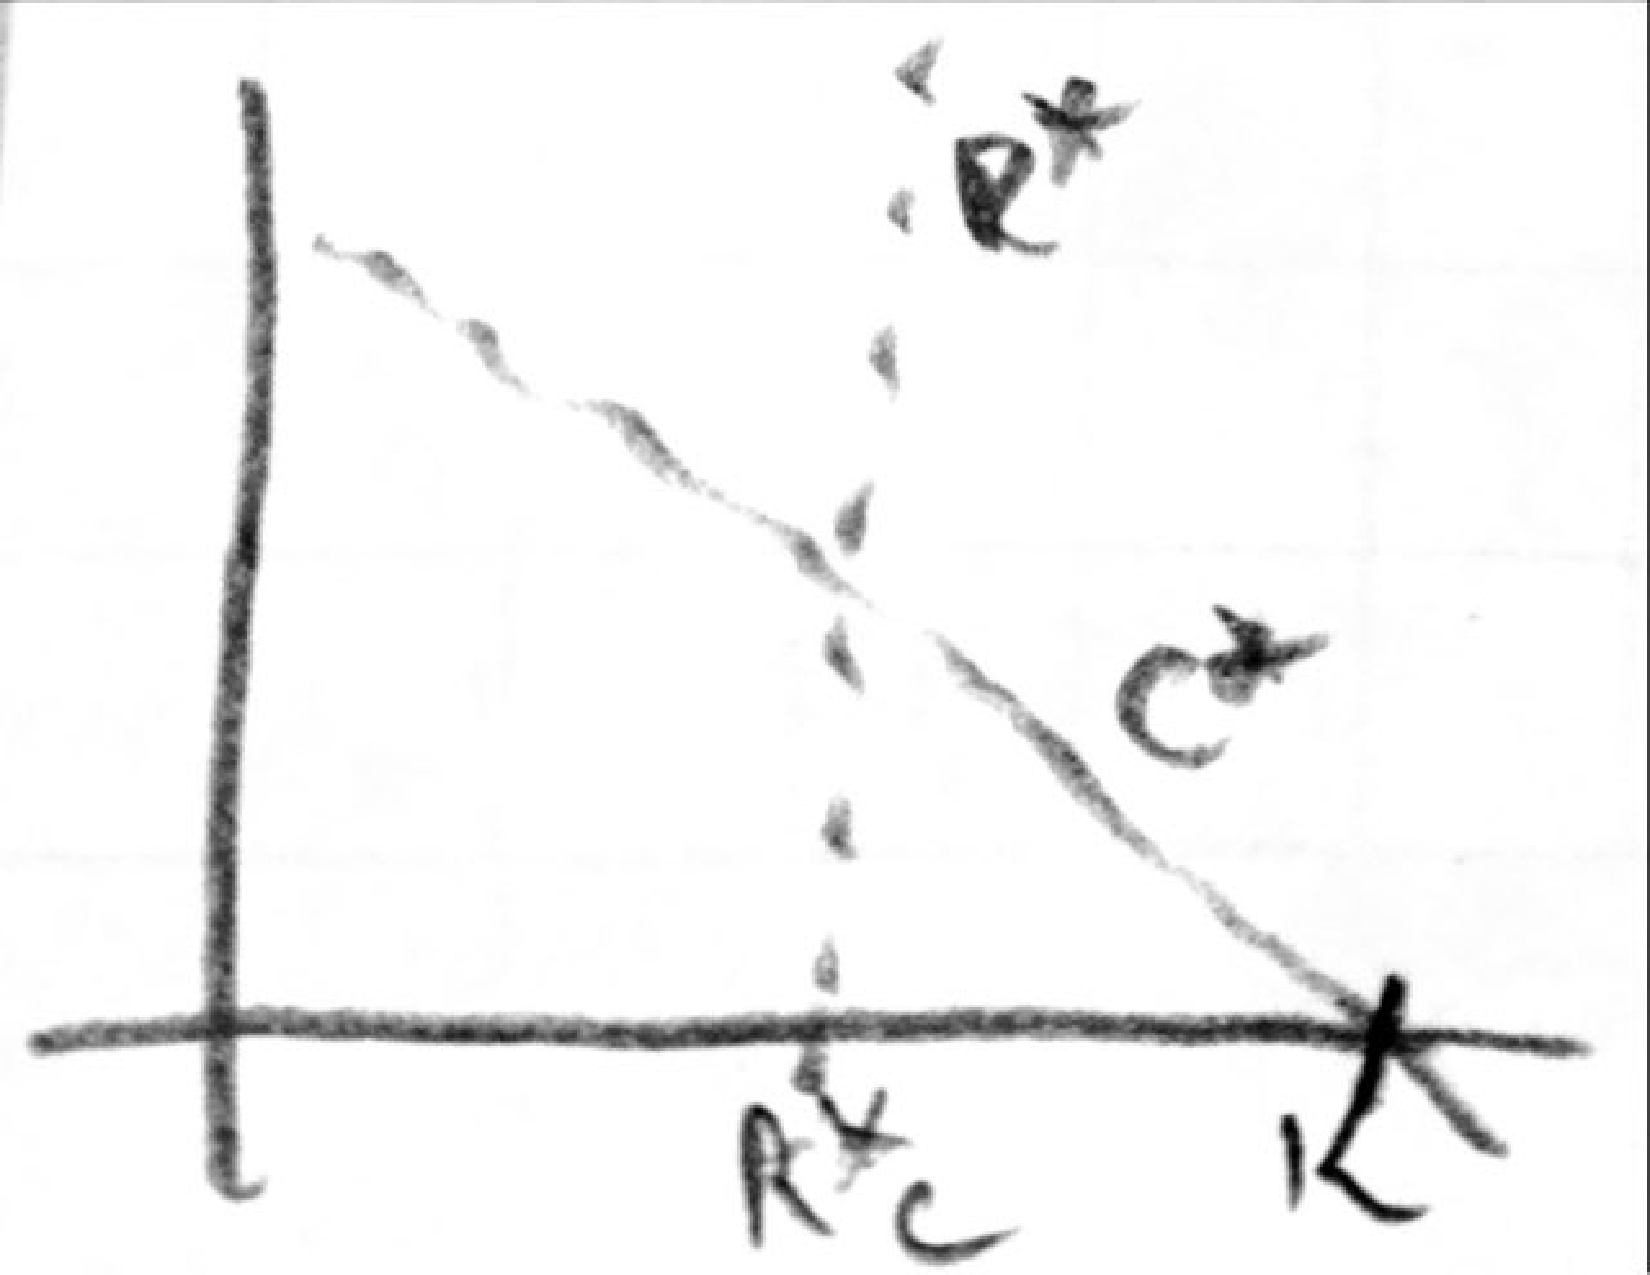
\includegraphics[width=3cm]{figs/TC.pdf}
\end{center}

\circled{4} $O$ can't invade $R$-only system.  When can $O$ invade an RC-system at equilibrium?\\
\ind RC equilibria:\\
\begin{align*}
	R_{eq}^*&=\frac{m_C}{a_{RC}e_{RC}}\\
	\\
	C_{eq}^*&= \frac{r-\frac{rR^*}{K}}{a_{RC}} = \frac{r-\frac{r\frac{m_C}{a_{RC}e_{RC}}}{K}}{a_{RC}} = \frac{r}{a_{RC}}-\frac{r m_C}{a_{RC}^2 e_{RC} K} = \frac{r(a_{RC}e_{RC}K-m_C)}{a_{RC}^2 e_{RC} K}
\end{align*}
\ind Invasion threshold $C_O^*$:
\begin{align*}
	\frac{1}{O}\frac{dO}{dt}=0 \qquad \Rightarrow \qquad C_O^* = \frac{m_O}{e_{CO}a_{CO}}
\end{align*}

\ind When does invasion threshold equal equilibrium (ie. $C_O^* = C_{eq}^*$)?
\begin{align*}
	C^* = \frac{m_O}{e_{CO}a_{CO}} &= \frac{r(a_{RC}e_{RC}K-m_C)}{a_{RC}^2 e_{RC} K}\\
	m_O a_{RC}^2 e_{RC} K &= e_{CO} a_{CO} r a_{RC} e_{RC} K - e_{CO} a_{CO} r m_C\\
	m_O a_{RC}  & = e_{CO} a_{CO} r - \frac{e_{CO} a_{CO} r m_C}{a_{RC}e_{RC} K}\\
	\frac{m_O a_{RC}}{e_{RO} a_{RO}}  & = r - \frac{ r m_C}{a_{RC}e_{RC} K}\\
	\Rightarrow & \quad   r - \frac{ r m_C}{a_{RC}e_{RC} K} - \frac{m_O a_{RC}}{e_{RO} a_{RO}}  \geq 0
\end{align*}
\begin{equation*}
\text{Invasion promoted by }\begin{cases}
\text{Higher productivity }(K)\\
\text{Higher conversion efficiencies }(e_{Ri})\\
\text{Lower mortality rates }(m_i)
\end{cases}
\end{equation*}
\ind \ind Note that conversion efficiencies and mortality rates contribute to \emph{`ecosystem efficiency'}\\
\ind \ind Effects of $r$ and $a_{RC}$ depend on mortality rates.\\

At what $K$ can $O$ invade?\\
\ind Solve $C_O^* - C_{eq}^* = 0$ for $K$
\begin{align*}
	m_O a_{RC}^2 e_{RC} K &= e_{CO} a_{CO} r a_{RC} e_{RC} K - r m_C e_{CO} a_{CO} \\
	K(m_O a_{RC}^2 e_{RC}-e_{CO} a_{CO} r a_{RC} e_{RC}) & =  - r m_C e_{CO} a_{CO} \\
	K  \geq   \frac{- r m_C e_{CO} a_{CO}}{(m_O a_{RC}^2 e_{RC}-e_{CO} a_{CO} r a_{RC} e_{RC})} & =  \frac{r m_C e_{CO} a_{CO}}{(e_{CO} a_{CO} r a_{RC} e_{RC}-m_O a_{RC}^2 e_{RC})}
\end{align*}

\note{Repeat with Mathematica}


\rule[0.5ex]{\linewidth}{1pt}

\begin{center}	\textbf{Intraguild predation} \end{center}
Contains exploitative competition, trophic chain \emph{and} apparent competition module!
\begin{align*}
		\frac{dO}{dt}&=e_{RO}a_{RO}R O + e_{CO}a_{CO}C O - m_o O\\
		\frac{dC}{dt}&=e_{RC}a_{RC}R C -a_{CO}CO- m_c C\\
		\frac{dR}{dt}&=r R \left(1-\frac{R}{K}\right) - a_{RC}RC - a_{RO}RO
\end{align*}
\circled{1}\circled{2}\\
Intuition from exploitative competition model:\\
\ind Invasion thresholds in absence of other consumer: 
\begin{align*}
		\frac{1}{O}\frac{dO}{dt} &= 0 \qquad \Rightarrow \qquad R_O^* =\frac{m_O}{e_{RO}a_{RO}}\\
		\frac{1}{C}\frac{dC}{dt} &= 0 \qquad \Rightarrow \qquad R_C^* =\frac{m_C}{e_{RC}a_{RC}}
\end{align*}

\ind If $K$ is low enough, $R$-only is stable. (i.e. if $K<\min(R_i^*)$)\\
\ind Consumer with lower $R^*$ invades first.
\circled{3}\circled{4}\\
If both consumers are present:
\begin{align*}
		\frac{1}{O}\frac{dO}{dt} &= 0 \qquad \Rightarrow \qquad R_O^* =\frac{m_O\boxed{-a_{CO}e_{CO}C}}{e_{RO}a_{RO}}\\
		\frac{1}{C}\frac{dC}{dt} &= 0 \qquad \Rightarrow \qquad R_C^* =\frac{m_C\boxed{+a_{CO}O}}{e_{RC}a_{RC}}
\end{align*}
Therefore, $C$ can never invade $RO$-equilibrium \emph{unless}...
\begin{equation*}
	\frac{m_C}{e_{RC}a_{RC}}<< \frac{m_O}{e_{RO}a_{RO}} 
\end{equation*}
\ind \ind \ind \ind \ind  ...which means that either $m_C << m_O$ and/or $e_{RC}a_{RC}>>e_{RO}a_{RO}$.\\

\textbf{Conclusion:}  Coexistence requires that IGprey is be superior competitor for shared resource.\\
\ind Otherwise $RO$-system occurs.\\

\circled{5}\\
When can $O$ invade stable $RC$-system?\\
\ind $RC$-system at equilibrium (exactly as for trophic chain):
\begin{align*}
	R_{eq}^*=\frac{m_C}{a_{RC}e_{RC}} \qquad \qquad 	C_{eq}^*= \frac{r(a_{RC}e_{RC}K-m_C)}{a_{RC}^2 e_{RC} K}
\end{align*}
\ind Invasion threshold\\
\begin{align*}
	\frac{1}{O}\frac{dO}{dt} = 0 \qquad \Rightarrow \qquad C_O^* = ... \textbf{\emph{  Mathematica}}
\end{align*}

\ind Solve $C_O^* - C_{eq}^* = 0 $ for $K$...\
\begin{align*}
	K \geq \frac{a_{CO}e_{CO}m_C r}{ a_{RC}(a_{RO}e_{RO}m_C - a_{RC}e_{RC}m_O + a_{CO}e_{CO}e_{RC}r)}
\end{align*}

\note{Show in Mathematica}\\

\circled{6}\\
When does $C$ go extinct at high $K$?\\
\ind Solve $C_{eq}^* = 0$ from $RCO$-equilibrium for $K$:\\
\begin{equation*}
	K \geq \frac{a_{CO}\overbrace{\phantom{e_{CO}}m_O} r}{ \underbrace{a_{RO}}(a_{RO}e_{RO}m_C - a_{RC}e_{RC}m_O + a_{CO}e_{CO}\underbrace{\phantom{e_{RC}}}r )}
\end{equation*}


\rule[0.5ex]{\linewidth}{1pt}

\begin{center}	\textbf{Temporal niche partitioning} \end{center}
Conclusion from exploitative competition model: $n\geq 2$ consumers cannot coexist on 1 resource.\\
But, among assumptions of this model was that interactions were linear.\\

Add Type II functional response to one of the two consumers.
\begin{align*}
	\frac{dO}{dt}&=e_{RO}\frac{a_{RO}R O}{1+a_{RO}h_{RO}R} - m_o O\\
	\frac{dC}{dt}&=e_{RC}a_{RC}RC - m_c C\\
	\frac{dR}{dt}&=r R \left(1-\frac{R}{K}\right) - a_{RC}RC - \frac{a_{RO}R O}{1+a_{RO}h_{RO}R}RO
\end{align*}
\note{$\Rightarrow$ Mathematica}
Handling time induces a lag, which induces cycles.\\
Cycles of $RO$ system induces cycles in $C$\\
\ind $C$ utilize resource when $O$ is at low abundance and $R$ is high. 

Armstrong \& McGehee also showed that $n \geq 4$ consumers can coexist on 4 resources.

\rule[0.5ex]{\linewidth}{1pt}





\end{document}